%% ===========================================================================
\FloatBarrier
\section{Validation and limiting cases}
\label{sec:verification}
%% ===========================================================================

\FloatBarrier
\subsection{Material, geometry and discretization}
\label{sec:material}

The parameters that the four cases of this section share are fixed once here,
so that each case varies only the feature it is meant to test; the material is
tetragonal $\mathrm{BaTiO_3}$ at room temperature, with the constants of
Table~\ref{tab:params}.

The dielectric anisotropy ratio
$\kappa_{11}/\kappa_{33}=39$ is retained, so the two poling configurations
differ in their permittivity as well as in their modulus. The strain-gradient
length scale is set by the window: with half-widths
$a_1\times a_2=3\times1$\,\si{\micro\meter} the cuboid window of
\eqref{eq:Mshapes} gives $M_{11}=3.0\times10^{-12}$ and
$M_{22}=3.3\times10^{-13}$\,\si{\square\meter}, that is characteristic lengths
$\sqrt{M_{11}}=\SI{1.73}{\micro\meter}$ and
$\sqrt{M_{22}}=\SI{0.58}{\micro\meter}$ along and across the strip. The ratio
$a_1/L=0.015$ is far inside the assumed operating range $a/L\le0.2$ of
Sec.~\ref{sec:limit_window}, using the inputs of Sec.~\ref{sec:formulation}.
The density $\rho$ rescales every frequency by the common factor
$1/2\pi\sqrt{\rho}$ and therefore moves the kilohertz numbers without touching
any ratio. The flexoelectric coefficient $\mu$ enters every
flexoelectric energy linearly and every flexoelectric coupling as $\mu^{2}$,
so the growth factors and the comparison with the piezoelectric response stand
whatever its value, while the absolute flexoelectric coupling follows it
quadratically.

\FloatBarrier
\subsection{Case I: benchmarks and mesh convergence}

The first case asks whether the element reproduces answers that are known
independently of it, and at what mesh the answers stop moving; the full record
of benchmarks, identities and independent routes is \ref{app:verification}.
In every case the solver assembles the weak form \eqref{eq:weak} with the
Hermite interpolation \eqref{eq:interp}, applies the kinematic conditions
\eqref{eq:bcmech}, and returns the higher-order stress \eqref{eq:sig} from the
constitutive relations of \eqref{eq:govexp}.

Three problems with known answers were solved with the same element: a
one-dimensional strain-gradient bar, whose static tip displacement and
frequency were compared with the closed form; the same bar in the classical
limit; and the constant-strain patch test. The clamped-free and clamped-clamped
frequencies of the strip agree with the Euler--Bernoulli values to $0.26\,\%$
and $0.10\,\%$, and the elastic strip reproduces the gradient theory whenever
the window is set to zero. Figure~\ref{fig:convergence} then shows the error in
the frequency of the extensional mode and in its quasi-static coupling factor
against the number of degrees of freedom. Both converge from above at the rate
expected of a bicubic Hermite interpolation, and the $48\times4$ mesh used
throughout the paper is inside the asymptotic range: refining it to $96\times4$
changes the frequency by $0.05\,\%$ and the coupling factor by $0.03\,\%$,
while the coarser $24\times2$ mesh used for the parameter sweeps differs from
it by $0.04\,\%$ and $0.03\,\%$. Table~\ref{tab:convergence} lists the four
meshes.

\begin{figure}[!htbp]
\centering
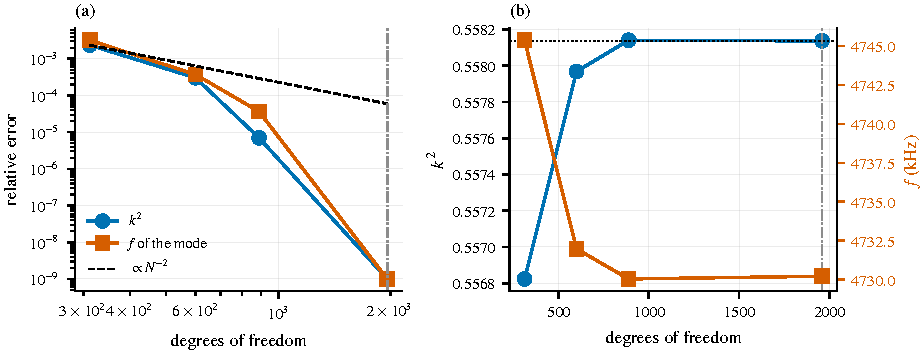
\includegraphics[width=\textwidth]{F2_convergence.pdf}
\caption{Variations of (a) the relative error of the extensional coupling factor $k^2$ and of the frequency of the mode that carries it, both referred to the finest mesh, and of (b) the two quantities themselves, against the number of mechanical degrees of freedom. The line in (a) is the $N^{-2}$ rate of a bicubic Hermite interpolation, the dotted line in (b) the converged value, and the $48\times4$ mesh is marked. The strip uses the material and geometry of Table~\ref{tab:params}, poling along $x$, plane stress and zero window size.}
\label{fig:convergence}
\end{figure}

\subsection{Case II: the coupling factor and its closed form}

The second case asks whether the assembled model reproduces the constitutive
coupling factor, which is the one quantity here that can be obtained without a
mesh.

The coupling factor of the extensional electrode pair is the one quantity in
this paper that can be obtained without a mesh, and doing so fixes the meaning
of every assembled value that follows. From the constitutive tensors alone,
\begin{equation}
  x=\frac{e^{\mathsf T}C_{p}^{-1}e}{\kappa}=1.2768,
  \qquad
  k^{2}=\frac{x}{1+x}=0.5608 ,
  \label{eq:xclosed}
\end{equation}
which is the closed-form value for the plane-stress strip; the
three-dimensional free bar gives $0.5771$, the three-dimensional uniaxial case
$0.3748$ and the two-dimensional plane-strain case $0.5132$, all from the same
tensors and all listed in \ref{app:data}. The plane-stress value is
the relevant one, because the strip is free out of plane.

The assembled model returns three numbers that belong to this same closed
form and differ from it for stated reasons. With the window switched off and
the strip unconstrained, the assembled route reproduces \eqref{eq:xclosed} to
$1.2\times10^{-11}$ relative, at $0.56079$: that is the validation of the
assembly, a comparison of two computations of one number. Clamping the left edge lowers the coupling to $0.55957$,
because the clamp restrains the in-plane deformation that carries the
piezoelectric charge, and switching the window on lowers it further to
$0.55814$, because the gradient stiffness adds energy to the same mode without
adding charge. The working value quoted in the abstract is the last of the
three, $k^{2}=0.5581$, which is $0.4\,\%$ below the free-strip closed form and
is the value a clamped device actually has. The two mode-based values,
$k^2_4=0.4650$ on the elastic memory matrix and $k^2_4=0.4583$ on the
short-circuit stiffness, are different measures again and are introduced where
the ring-down uses them (Sec.~\ref{sec:memorystudy}); they are not comparable
with the mode-free ones and are never averaged with them.

\subsection{Case III: time discretization and the step used}

The third case asks whether the L1 march converges at the order the scheme
promises and which step the ring-downs later use.

The L1 scheme is first order in $\Delta t$ for every $\alpha\in(0,1]$, at
$\alpha=1$ as well. At $\alpha=1$ and $\omega\tau=0.3$ the damping ratio
extracted from the ring-down is $0.150111$, $0.150057$ and $0.150029$ at $N$,
$2N$ and $4N$ steps over twenty periods ($N=12000$, that is $600$ steps per
period), against the exact $\omega\tau/2=0.150000$: halving the step halves the
residual, an observed order of $0.97$, and the sequence extrapolates to the
exact value. The ring-downs of Sec.~\ref{sec:memorystudy} are run at the $4N$
step. The eight curves of Sec.~\ref{sec:transient} are a coarser march, $400$
steps per period, and their decrements carry the step in the last decimal.

\subsection{Case IV: the fields of the coupled bending mode}

The fourth case asks whether the coupled solution has the spatial structure
the constitutive model implies: a bending mode that is electrically silent in
the piezoelectric sense, and a through-thickness strain gradient that is not.

Figure~\ref{fig:fields} records the four fields of the coupled bending mode in
the open-circuit configuration, together with the strain gradient that drives
the flexoelectric term. The in-plane and the transverse displacement are those
of a first bending mode; the potential is not. It reaches tens of millivolts a
few tens of micrometers from the clamped edge and near mid-height, and falls
toward both the edge and the free end, so the two face electrodes sit where the
potential is smallest. That is the spatial form of the cancellation that makes
this configuration insensitive to the piezoelectric charge and responsive to
the strain gradient, and the gradient panel shows where the flexoelectric
charge is generated: in the boundary layer at the clamp and along the neutral
axis, not at the electrodes.

\begin{figure}[!htbp]
\centering
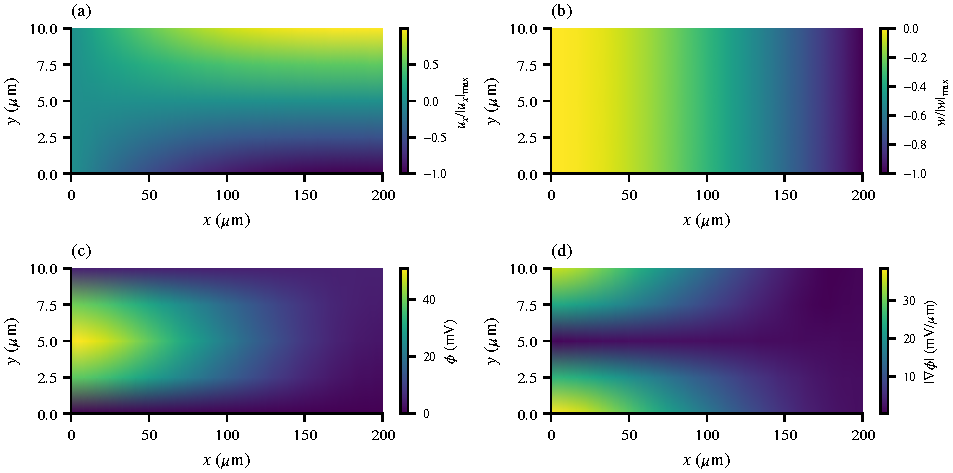
\includegraphics[width=\textwidth]{F3_fields.pdf}
\caption{Variations of (a) the in-plane displacement, (b) the deflection, (c) the potential at \SI{10}{\nano\meter} of tip motion, (d) the electric field and (e) the magnitude of the strain gradient that drives the flexoelectric term over the coupled bending mode, in the open-circuit configuration on a $48\times4$ mesh, with the geometry, material and window of Table~\ref{tab:params}, poling along $y$ and plane stress. The potential is smallest at the face electrodes and the gradient largest at the clamp.}
\label{fig:fields}
\end{figure}

\FloatBarrier
\subsection{The worked calculation of the headline numbers}
\label{sec:worked}

The numbers quoted in the abstract follow from the inputs in four short steps,
collected here so that the route from a material constant to a coupling factor
is visible and not only its outcome; Table~\ref{tab:worked} lists inputs and
outputs side by side.

\paragraph{Window} For half-widths $a_1=\SI{3}{\micro\meter}$ and
$a_2=\SI{1}{\micro\meter}$ the second-moment tensor of the cuboid window is
diagonal with
\begin{equation}
  M_{11}=\frac{a_1^{2}}{3}=3.000\times10^{-12}\ \si{\meter\squared},\qquad
  M_{22}=\frac{a_2^{2}}{3}=3.333\times10^{-13}\ \si{\meter\squared},
  \label{eq:Mnumber}
\end{equation}
an anisotropy ratio $M_{11}/M_{22}=9$. The three shapes are interchangeable
once $M$ is fixed, because $M_{ii}=a_i^{2}/3$, $a_i^{2}/4$ and $a_i^{2}/5$ for
the cuboid, the ellipse and the ellipsoid: an ellipsoid of half-width
$a_{\rm ell}=1.2910\,a_{\rm cub}=\sqrt{5/3}\,a_{\rm cub}$ reproduces
\eqref{eq:Mnumber} exactly, and the reciprocal
$a_{\rm cub}=0.7746\,a_{\rm ell}$ is the conversion used for the equal-$M$ pair
of Sec.~\ref{sec:windowshape}.

\paragraph{Plane-stress reduction and closed form} The strip is free out of
plane, so the stiffness that multiplies $\varepsilon_{xx}$ is the reduced entry
\eqref{eq:Cp}, which for $\mathrm{BaTiO_3}$ gives
$C^{p}_{xx}=9.5500\times10^{10}$\,Pa with the poling along $x$ and
$1.6946\times10^{11}$\,Pa with the poling along $y$, and
$C^{p}_{12}=5.7000\times10^{10}$\,Pa in both cases. The entries that pair with
it are $e_{33}=6.7$ and $e_{31}=-0.7$\,\si{\coulomb\per\square\meter} and the
permittivity across the electrode gap,
$\kappa_{yy}=\kappa_{33}=4.9583\times10^{-10}$\,\si{\farad\per\meter}. Hence
$x=1.2768$ and $k^{2}=0.5608$ from \eqref{eq:xclosed}, with no mesh involved.

\paragraph{Assembled route} The same quantity on the assembled model comes from
one short-circuit and one open-circuit reduction of the $48\times4$ mesh:
$245$ nodes, eight mechanical degrees of freedom per node ($1960$ unknowns)
and $245$ potential unknowns, condensed to a single electrode pair $(d,\beta)$
with $\beta=2.4792\times10^{-11}$\,\si{\farad}. Then
\begin{equation}
  x_{\rm FEM}=\frac{d^{\mathsf T}K_{sc}^{-1}d}{\beta}=1.2631,
  \qquad
  k^{2}_{\rm FEM}=\frac{x_{\rm FEM}}{1+x_{\rm FEM}}=0.5581 ,
  \label{eq:xFEM}
\end{equation}
$0.47\,\%$ below \eqref{eq:xclosed}; the clamped edge accounts for $0.22\,\%$
of that and the gradient stiffness for a further $0.26\,\%$.

\paragraph{Flexoelectric smallness and L1 weights} With the piezoelectric
constants switched off, the same reduction gives the smallness parameter of the
bending configuration,
\begin{equation}
  x=\frac{3\mu^{2}}{C^{p}_{xx}\,h^{2}\,\kappa_{33}}
   =\frac{3\,(10^{-6})^{2}}{1.6946\times10^{11}\cdot(10^{-6})^{2}\cdot
     4.9583\times10^{-10}}
   =3.5704\times10^{-4}
  \label{eq:xflexo}
\end{equation}
at $h=\SI{10}{\micro\meter}$, against a finite element value of
$1.7437\times10^{-4}$; the two routes differ by a factor $2.05$ and the
difference is discussed with the thickness sweep in Sec.~\ref{sec:thickness}.
The L1 weights are fixed numbers that do not depend on the model,
\begin{equation}
  \alpha=0.5:\; (b_0,b_1,b_2)=(1,\;0.414214,\;0.317837),\qquad
  \alpha=0.7:\; (b_0,b_1,b_2)=(1,\;0.231144,\;0.159245),
  \label{eq:bweights}
\end{equation}
and the damping ratio follows from the decrement of two successive peaks,
\begin{equation}
  \delta=\ln\frac{A_k}{A_{k+1}},\qquad
  \zeta_{\rm eff}=\frac{\delta}{\sqrt{4\pi^{2}+\delta^{2}}} ,
  \label{eq:zeta}
\end{equation}
of which $\zeta=\delta/2\pi$ is the small-damping approximation. At
$\omega\tau=0.3$ the ratio of two successive voltage peaks is $2.5947$, so
$\delta=0.95345$ and $\zeta_{\rm eff}=0.15003$ against the exact
$\omega\tau/2=0.15000$.

%% Summary of the worked calculation: inputs -> intermediate -> output.
\begin{table}[!htbp]
\centering
\small
\caption{The headline numbers of the abstract, from their inputs. Each value
is the one carried into the figures and tables of this section; the last column
is the number the abstract quotes.}
\label{tab:worked}
\begin{tabular}{@{}p{0.20\textwidth}p{0.22\textwidth}p{0.24\textwidth}p{0.24\textwidth}@{}}
\toprule
quantity & inputs & intermediate & value \\
\midrule
extensional coupling & $C_p$, $e$, $\kappa_{33}$ &
$x=1.2768$; $x_{\rm FEM}=1.2631$ & $0.5581$ ($0.5608$ closed form) \\
thickness independence & $k^2$ at $10$ and \SI{1}{\micro\meter} &
$0.55814\to0.55861$ & $0.09\,\%$ \\
flexoelectric growth & $\mu$, $C^{p}_{xx}$, $h$, $\kappa_{33}$ &
$1.7437\times10^{-4}\to4.1736\times10^{-3}$ & factor $24$ \\
flexoelectric slope & the eight thicknesses & local log--log slopes &
$-1.96$ to $-0.43$ \\
window anisotropy & $M_{11}$, $M_{22}$, $\theta$ & $M$ rotates, the mesh does
not & $15$--$19\,\%$ \\
two configurations & \eqref{eq:xclosed} in both & $0.4580$ against $0.1141$;
\SI{138.99}{\volt} against \SI{2.41}{\volt} & factor $58$ \\
memory ratio & $K_{\rm eff}$, $K_{uu}$ & $\zeta=0.15003$ against $0.06746$ &
$0.450$ \\
integer-order limit & $\omega\tau=0.3$ & $\zeta_{\rm eff}$ against
$\omega\tau/2$ & $0.02\,\%$ \\
\bottomrule
\end{tabular}
\end{table}


The four cases and the worked calculation fix the input set of the paper: the
material constants of Table~\ref{tab:params}, the window of
Sec.~\ref{sec:material} and the mesh sizes named above. With them the
quantities of Sec.~\ref{sec:results} follow, and each of those results is
reported below as a figure, a mechanism and a number.

\FloatBarrier
